\documentclass{article}
\usepackage[utf8]{inputenc}
\usepackage[margin=1in]{geometry}
\usepackage{booktabs}
\usepackage{tabu}
\usepackage[labelfont=bf, skip=5pt, font=small]{caption}
\usepackage[]{subcaption}
\usepackage{graphicx}
\usepackage{fancyhdr}
\usepackage{amsmath}
\usepackage{float} % here for H placement parameter
\usepackage{hyperref}
\usepackage{siunitx}

\font\myfont=cmr12 at 100pt
\title{\Huge DATA304 Project Group 4:\\
  \Huge A study of the LAB cafe at Victoria University}
\author{\Large Kevin Ye, Vivian Dong, Patrick Quito, Tama Hoare }
\date{\Large May 2022}

\begin{document}


\maketitle
\newpage

\section{Introduction}

\subsection{Description of LAB Cafe and the main objective of project}
The LAB Food and Beverage Co. is a Cafe located at ground level of the Easterfield Building at Kelburn campus of Victoria University of Wellington 6012, New Zealand. As part of a project for DATA304 course at Victoria University, our group decided to model this cafe system by analyzing customer interarrival time and service times. 

The cafe is open from 7.30am to 3pm every weekday. There are 3 servers by the counter ready to serve. The cafe sells a variety of coffee and brunch items such as rolls, sandwiches, salads, noodles etc. Servers serve customers by taking customer orders. Then they spend some time getting the customer's order ready. They finally call out the customer when their order is ready. The cafe's main customers are students and staff from Victoria University Kelburn Campus. 

The one of the main objectives of this project is to model the interarrival time and service times of customers by fitting a best fit distribution to these times. The other main objective is to develop SimPy models in Python to be able to simulate the cafe system and assess how good each model is.

\subsection{Customer interaction with the system - Vivian}
Customers need to choose one of the three counters to order and pay, and they will wait if there is a queue. Afer ordering they will stay in the café till the staff call their name means the order is ready.

\subsection{Process of data collection}
4 people collecting data
different days
approx 2 hours there collecting. Tama

\subsection{Process of data cleaning}
missing values 
getting the read data file to work. Patrick

Note: The structure of the git repository that contains this report and all other relevant files were structured according to here\cite{frery2020badging}.

\section{Data analysis}

\subsection{Fitting best fit distributions (Vivian)}

We tried to approximate "inter-arrival time" and "service time" using the following 12 Distributions: Weibull Minimum Extreme Value distribution, Normal distribution, Weibull Maximum Extreme Value distribution, Beta distribution, Inverse Gaussian distribution, Uniform distribution, Gamma distribution, Exponential distribution, Log-normal distribution, Pearson Type III distribution, Triangular distribution, Erlang distribution. After fitting different distributions, we checked the Goodness of fit based on Chi-square Statistics. The outputs for "inter-arrival time" sorted in order of Goodness of fit looks like this: 

\sisetup{round-mode = places, round-precision = 3}

\begin{table}[H]
    \caption{Distributions listed by Betterment of fit}
    \label{tab:Inter-arrival Best Fit}
    \begin{center}
    \begin{tabular}{c S}
        \toprule
        \textbf{Distribution} & \textbf{chi square}\\
        \midrule
        Pearson Type III distribution & 9.155\\
        Weibull Minimum Extreme Value distribution & 13.245\\
        Beta distribution & 21.708\\
        Log Normal distribution & 25.596\\
        Inverse Gaussian distribution & 29.390\\
        Exponential distribution & 29.515\\
        Gamma distribution & 48.359\\
        Triangular distribution & 209.930\\
        Normal distribution & 332.531\\
        Uniform distribution & 510.690\\
        Erlang distribution & 672.400\\
        Weibull Maximum Extreme Value distribution & 1137.915\\
        \bottomrule
    \end{tabular}
    \end{center}
\end{table}

The outputs for "service time" sorted in order of Goodness of fit looks like this:


\begin{table}[H]
    \caption{Distributions listed by Betterment of fit}
    \label{tab:Service Best Fit}
    \begin{center}
    \begin{tabular}{c S}
        \toprule
        \textbf{Distribution} & \textbf{chi square}\\
        \midrule
        Beta distribution & 1.231338\\
        Weibull Minimum Extreme Value distribution & 2.831316\\
        Pearson Type III distribution & 4.130412\\
        Gamma distribution & 4.131762\\
        Erlang distribution & 4.132443\\
        Inverse Gaussian distribution & 10.560874\\
        Log Normal distribution & 11.688749\\
        Exponential distribution & 29.775131\\
        Triangular distribution & 39.441479\\
        Normal distribution & 140.194689\\
        Uniform distribution & 305.594183\\
        Weibull Maximum Extreme Value distribution & 1080.829277\\
        \bottomrule
    \end{tabular}
    \end{center}
\end{table}

The Chi-square statistics suggest that the Pearson Type III distribution best approximates 'inter-arrival time'. We can also see that Beta distribution is the best fit for 'service time'. The python code using the Scipy Library to fit the distribution is from here\cite{git} Suppose we had more time to do this part. In that case, we will add more distributions to fit our data and find a better fit distribution of the interarrival/service times. Furthermore, we can also use the Anderson-Darling test or other goodness-of-fit tests to compare whether we will get the same results.

\subsection{Histogram plots for visual evaluation (Patrick)}

\begin{figure}[H]
    \centering
    \begin{subfigure}[b]{0.45\textwidth}
        \centering
        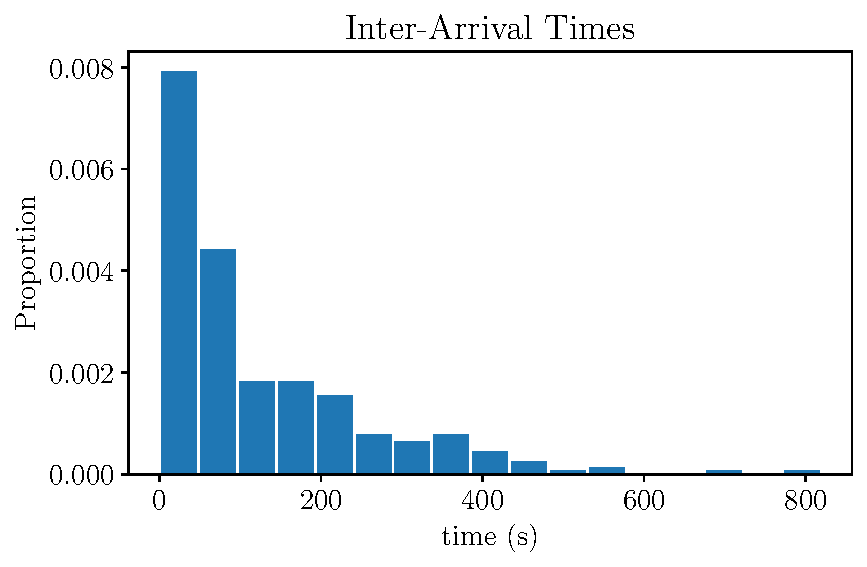
\includegraphics[width=\textwidth]{fig1.pdf}
        \caption{}
        \label{fig:img1}
    \end{subfigure}
    \hfill
    \begin{subfigure}[b]{0.45\textwidth}
        \centering
        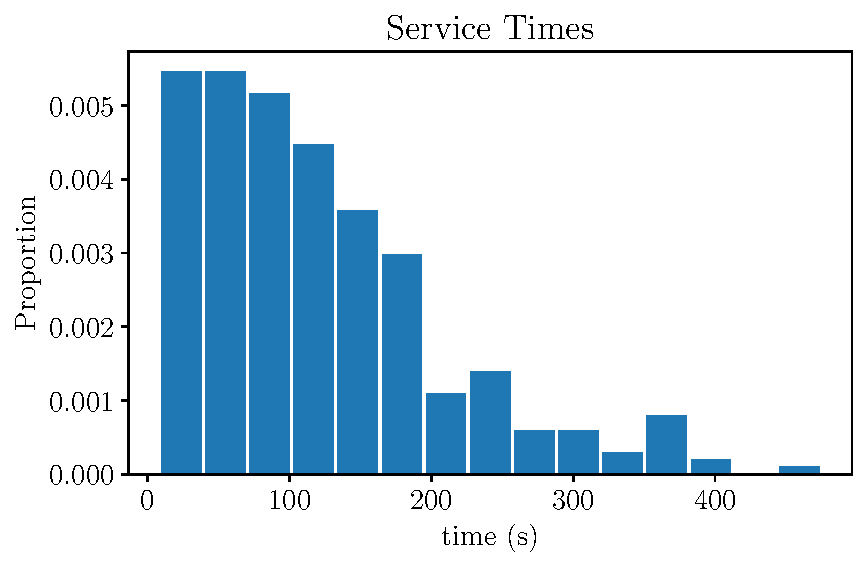
\includegraphics[width=\textwidth]{fig2.pdf}
        \caption{}
        \label{fig:img2}
    \end{subfigure}

    \caption{Histograms of inter-arrival times and service times}
    \label{fig:two-figs}
\end{figure}

Here, we have divided the inter-arrival time and the service time data into a number of phases, such that the time occupied by each phase has a negative exponential distribution. This is used by Erlang regarding service to be completed in k phases which has the same negative-exponential distribution, thus obtaining what is called a k-Erland distribution.
The inter-arrival is the interval of time between each arrival. Assuming that the arrivals are independent, their distribution is exponential.
The service times defines as the time required to serve a customer. 
These assumptions are further confirmed above by the histograms of the observations. We have observed the arrival of customers for a few hours.

\begin{figure}[H]
    \centering
    \begin{subfigure}[b]{0.45\textwidth}
        \centering
        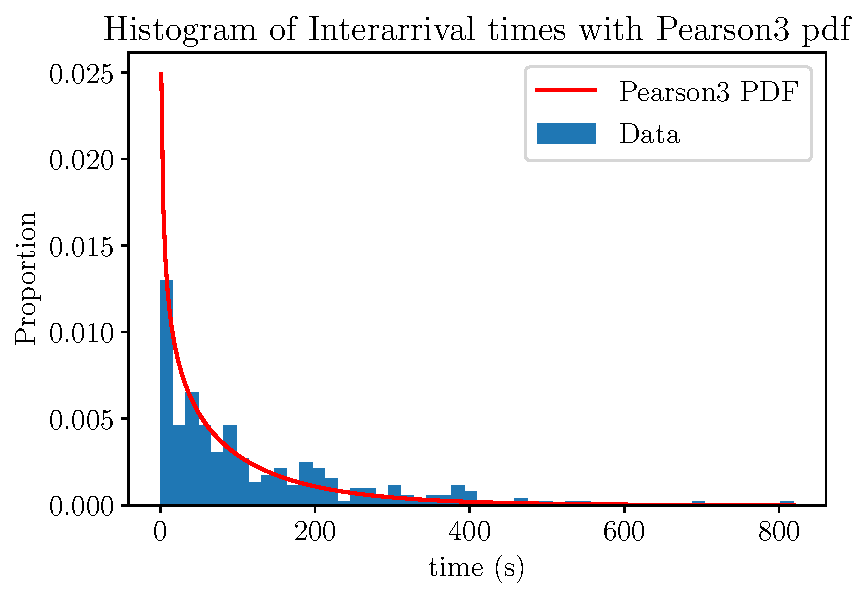
\includegraphics[width=\textwidth]{fig3.pdf}
        \caption{}
        \label{fig:img3}
    \end{subfigure}
    \hfill
    \begin{subfigure}[b]{0.45\textwidth}
        \centering
        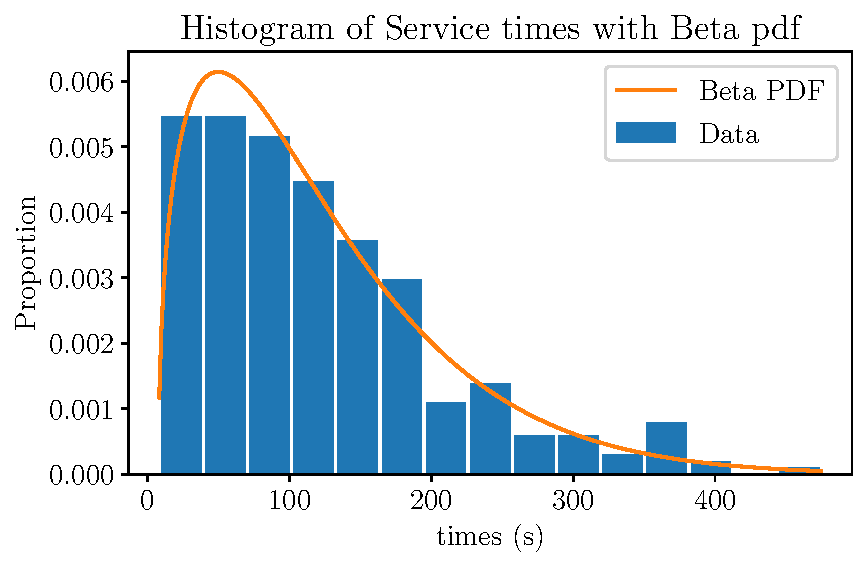
\includegraphics[width=\textwidth]{fig4.pdf}
        \caption{}
        \label{fig:img4}
    \end{subfigure}

    \caption{Histograms with best fit distribution pdf overlayed}
    \label{fig:two-figs2}
\end{figure}

The second pair of histograms above are fitted with the best fit distributions. We have fitted the inter-arrival and service time histograms with a list of distributions listed by Betterment of fit. Based on the Chi-square Statistics, it suggests that Pearson3 is the best in approximating ‘inter-arrival time’ Data. For our 'service times' data, it suggests that beta distribution is the best fit for the data.

\section{Simulation models}

\subsection{Performance Measures of collected data (Tama)}

\begin{table}[H]
    \centering
    \caption{This is the caption that goes at the top of the table}
    \begin{tabu}{X S}
        \toprule
        \textbf{Performance Measures} & \textbf{Values calculated from data}\\
        \midrule
        Average time in system (seconds), $W$   & 140.07 \\
        Average number of customers in the system, $L$ & 1.1819\\
        Proportion of time servers are busy, $B$ & 0.61148  \\
        Effective arrival rate (per second), $\lambda_{\text{eff}}$ & 0.0084381\\
        \bottomrule
    \end{tabu}
    \label{tab:Original Data PF}
\end{table}

Assessing the performance measures of the collected data is key modelling the performance of the servicing unit. As shown in the tables above there were seven key performance measures assessed from the collected data. 

Firstly, we can see that the average time that a customer spent at the café service unit, meaning the total time of queuing plus service, was 140,07 seconds. The average number of customers in the system at any given point was 1.18. We can see from the data that the server at the café was busy serving customers 61.15% of the time. The remaining time is spent with no customers being served at the café.

The performance measure of effective arrival rate corresponds to the rate at which customers enter the service unit. We can see that 0.0084 customers entered the café per second. The correlates to 30.38 customers coming to the café per hour.

\begin{table}[H]
    \centering
    \caption{This is the caption that goes at the top of the table}
    \begin{tabu}{X S}
        \toprule
        \textbf{Other parameters} & \textbf{Values calculated from data} \\
        \midrule
        Average Inter-arrival time $\frac{1}{\lambda}$ (seconds) & 120.32945045312502  \\
        Average Service time, $W_s$ (seconds) & 120.77890398148169  \\
        Average Queue Time, $W_q$ (seconds) & 19.29576795987645  \\
        \bottomrule
    \end{tabu}
    \label{tab:Original Data Other}
\end{table}

The average inter-arrival time is the average time difference between arrival of one customer and then the next customer. It is a time elapse between the arrival of the person and one following it in the queue. The value calculated from this in the data was 120.33 seconds.

The time it takes for one customer to be served is referred to as the service time. This is the time between a single customer reaching the server (no longer in the queue) and leaving the service unit. Hence it took on average 120.77s for a customer to be served at the café once they had reached the server.

The average queue time is the time between a customer arriving at the service system and getting to the point at which they start to get served. They spend that time in a queue. At the café it took on average 19.295 seconds for a customer to get to the server once they had arrived at the café. Hence they spent of average 19.295 seconds in a queue at the café.




\subsection{M1 model (Patrick)}

The M1 model is a task where we investigate and use either M/M/1 or M/M/C depending on our structure. An M/M/1 queue represents the queue length in a system having a single server, where arrivals are determined by a Poisson process and service times gave an exponential distribution. In the case of our project, we have an M/M/3 queue as there were 3 servers from where we gathered our data form.

$$
\pi_{0} = \frac{1}{\sum_{k=0}^{s-1}{\frac{\rho^k}{k!}} + \frac{\rho^s}{s!}\frac{1}{1-\frac{\rho}{s}}}
$$

$$
\pi_{0} = \frac{1}{\frac{\rho^0}{0!} + \frac{\rho^1}{1!} + \frac{\rho^2}{2!} + \frac{\rho^3}{3!}\frac{1}{1-\frac{\rho}{3}}}
$$

$$
\pi_{0} = \frac{1}{1 + \rho + \frac{\rho^2}{2} + \frac{\rho^3}{6}\frac{1}{1-\frac{\rho}{3}}}
$$

$$
\pi_{0} = 0.369
$$

$$
B = 1-\pi_{0} = 0.631
$$

$$
L = \pi_{0}\frac{\frac{\rho^{s+1}}{s!s}}{(1-\frac{\rho}{s})^2}+\rho
$$

$$
L = \pi_{0}\frac{\frac{\rho^{4}}{3!3}}{(1-\frac{\rho}{3})^2}+\rho
$$

$$
L = 1.034
$$

$$
W = \frac{L}{\lambda} = 124.390
$$

Mathematics used were from works published on operations research\cite{hillier1967introduction}\cite{little1961proof}

Upon generating all the values (check the table below), we have used the formula to compare to the original data we’ve gathered. This is used to confirm that the values from the M1 model are correct after doing the math.

The log relative error is one of the easiest way to compare 2 numbers. See here\cite{almiron2010numerical} for more detail on how to use LRE, published by one of our lecturers, Alejandro.

The LRE is defined as 

$$
LRE(x,c)=\begin{cases}
    -\log_{10}{\frac{|x-c|}{|c|}}, & \text{if $c \neq 0$}.\\
    -\log_{10}{|x|}, & \text{otherwise}.
\end{cases}
$$

\begin{table}[H]
    \centering
    \caption{Comparing performance measures of Collected data and M1 model}
    \begin{tabu}{X S S S}
        \toprule
        \textbf{Performance Measures} & \textbf{Collected Data} & \textbf{M1 model}& \textbf{LRE}\\
        \midrule
        Average time in system (seconds), $W$ & 140.07467194135813 & 124.33303596116097 & 0.9493097487424857\\
        Average number of customers in the system, $L$ & 1.1819665982792091 & 1.0435912057915153 & 0.9315463380768094\\
        Proportion of time servers are busy, $B$ & 0.6114848739024165 & 0.641133566988506 & 1.314380164078804\\
        Effective arrival rate (per second), $\lambda_{\text{eff}}$ & 0.008438117911666687 & 0.00839529474026536 & 2.2945667626263146\\
        \bottomrule
    \end{tabu}
    \label{tab:M1}
\end{table}

In creating the M1 model, we took inspiration from the assignments and labs to be able to produce these outcomes. We have passed our data on arrival and service rate through the model and got the values above.
We had a mean arrival rate of 0.008310517468785045 per second, and a mean service rate of 0.008279591609419837 per second. The LAB Cafe is open from 7:30 am to 3:00 pm a total of 7.5 hours per day which is equivalent to 27000 seconds which would be the max time of each simulation. 
W is denoted as the average waiting of customers, L is the average number of customers in the system, B is the proportion of time that servers are busy, and lambdaEff is the effective arrival rate.

\subsection{M2 model (Vivian)}

The M2 model is a simulation model developed using SimPy to model the LAB cafe customer waiting and serving system. M2 model uses the interarrival times best fit distribution (Pearson3) and the service times best fit distribution (Beta) to simulate the performance. Below is the comparison between the original data performance measure estimates and the performance measures estimates produced by M2 model.

\begin{table}[H]
    \centering
    \caption{Comparing performance measures of Collected data and M2 model}
    \begin{tabu}{X S S S}
        \toprule
        \textbf{Performance Measures} & \textbf{Collected Data} & \textbf{M2 model}& \textbf{LRE}\\
        \midrule
        Average time in system (seconds), $W$ & 140.07467194135813 & 143.28751362199432 & 1.6394702886840742\\
        Average number of customers in the system, $L$ & 1.1819665982792091 & 1.6283817237073634 & 0.4228663028617897\\
        Proportion of time servers are busy, $B$ & 0.6114848739024165 & 0.7140026917524969 & 0.7755863651011485\\
        Effective arrival rate (per second), $\lambda_{\text{eff}}$ & 0.008438117911666687 & 0.011347266899941985 & 0.4624796261431971\\
        \bottomrule
    \end{tabu}
    \label{tab:M2}
\end{table}

From the table above, we can see that the estimated W from the M2 model has a difference of approximately 3.21 from the estimate provided by the original data collected. The L difference between the two estimations by the collected data and the M2 model is about 0.45. The difference in the proportion of time servers are busy (B) was 0.1 between the two estimates of the collected data and the M2 model. The effective arrival rate $\lambda_{\text{eff}}$ has a difference of 0.0029 approximately between the original data and the M2 estimate. We can see that the M2 model is a decent fit for the actual data as the differences are relatively small.



\subsection{M3 model (Kevin)}

\begin{table}[H]
    \centering
    \caption{Comparing performance measures of Collected data and M3 model}
    \begin{tabu}{X S S S}
        \toprule
        \textbf{Performance Measures} & \textbf{Collected Data} & \textbf{M3 model}& \textbf{LRE}\\
        \midrule
        Average time in system (seconds), $W$ & 140.07467194135813 & 127.14403384042575 & 1.0347396570447596\\
        Average number of customers in the system, $L$ & 1.1819665982792091 & 1.0853339772074488 & 1.0874814442563059\\
        Proportion of time servers are busy, $B$ & 0.6114848739024165 & 0.6246586034558348 & 1.6666769750434784\\
        Effective arrival rate (per second), $\lambda_{\text{eff}}$ & 0.008438117911666687 & 0.00852846013566267 & 1.9703548122023773\\
        \bottomrule
    \end{tabu}
    \label{tab:M3}
\end{table}

The M3 model is a simulation model developed using SimPy to model the LAB cafe customer waiting and serving system. The distribution of interarrival and service times are modelled after the empirical distributions of the interarrival times and services times recorded from the original data. From the M3 model produced some performance measures estimates in the table above which we can compare to the original data performance measure estimates to gauge how well of a fit this M3 model is at simulating the nature of the real life system.

From the table we can see that estimated W from the M3 model has a difference of approximately 13 to the estimate provided by the original data collected. The L difference between the two estimations by the colletced data and the M3 model is about 0.1. The difference in the B, proportion of time servers are busy was 0.01 between the two estimates of the collected data and the M3 model. The effective arrival rate $\lambda_{\text{eff}}$ has a difference of 0.0001 approximately between the original data and the M3 estimate. We can see that The M3 model is a decent fit for the original data as the differences are around about $10\%$ of the original data estimates.

\section{Conclusion}

\subsection{Results Summary}


\subsection{Improvements}
\subsection{}
\subsection{}


\bibliographystyle{plain}
\bibliography{references}

\end{document}
